
\section{Implementation}
Figure~\ref{fig:prototype_component_overview} describes interaction between the chatbot and the Facebook Messenger servers. The user interacts with the chatbot using the Facebook Messenger platform on either a mobile phone or website. When the user sends a message to the chatbot, it is sent via Facebook servers who decide where to forward the message onto. The message comes in a \textit{json} format that is parsed by the chatbot application to understand the content of the message and how the user interacted with the bot. For example, if the response is from a quick reply, then additional parameters are sent. The chatbot reads and writes the necessary information into a database to decide a response. When it is ready, it sends a request to the Facebook servers that forward it onto the user's Facebook Messenger account that can be read from the Messenger platform (Figure~\ref{fig:prototype_component_overview}). All code is open-source and hosted on \textit{GitHub} (\url{www.github.com/harrymt/harryshabits}).

\begin{figure}[H]
    \centering
    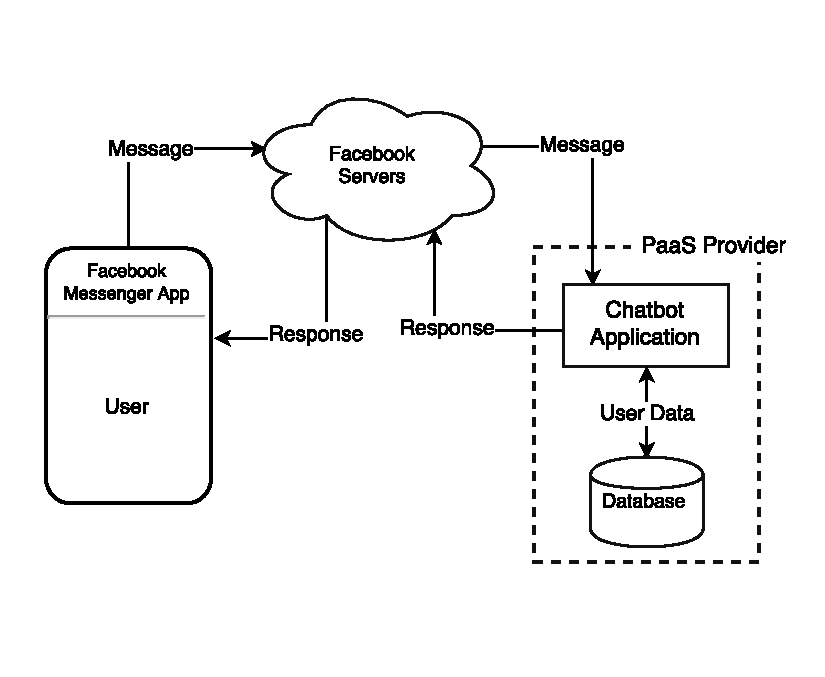
\includegraphics[width=5.1in]{../resources/diagrams/chatbot-component-overview.pdf}
    \caption{Interaction between a user and the chatbot application via Facebook servers.}
    \label{fig:prototype_component_overview}
\end{figure}

The prototype is written in JavaScript running on a \textit{node.js} (\url{www.nodejs.org}) server, built on the Facebook Messenger chatbot platform and hosted on \textit{Heroku} (\url{www.heroku.com}) --- a free PaaS (Platform-as-a-Service) option. Facebook Messenger encourages developers to create bots to interact with their users as these bots act as a real person with similar interaction flow, plus a few additional features, such as \textit{Quick Replies}~\cite{doc_fb_quick_replies} for revealing a list of options to a user. Simple call and responses were used to interact with users and track their data instead of natural language processing (NLP) to limit the scope of the project. Instead of natural language processing, the location of the bot (inside an existing messaging app) ease of interaction and the additional features (Quick Replies) help easily communicate with users.


Different languages, server, hosting provider and database provider were considered. JavaScript with node.js on Heroku with PostgreSQL were chosen because of the following reasons: node.js enables us to share the same language for the server and the client; large amount of packages to handle client and server side functionality; suitable for prototyping and rapid product iteration; Heroku has a free-tier which allows full deployment with a PostgreSQL database of up to 10,000 rows; Heroku hosts the application in the cloud, giving benefits for scalable deployments that benefit any potential future application growth. Finally, \textit{Airtable} (\url{www.airtable.com}) --- a database integration was integrated, however, it only provided 3,000 free rows and therefore was discarded in favour of Herokus PostgreSQL database.


\subsection{Database}
The bot tracked data about how people logged their habits, such as what day they tracked their habit and how many times they delayed their checking messages. Heroku provides 10,000 rows as their free option in a \textit{PostgreSQL} (\url{https://www.postgresql.org/}) database. Figure~\ref{fig:db_diagram} outlines each table in the database with what information is stored. The \textit{Facebook user ID} is used to identify each user and what habits they tracked. When a user has told the bot they completed their habit, a new row in the \textit{Habits} table would be added and linked to the user in the \textit{Users} table. Two global variables are used to maintain the state across local and live versions of the system to display the length of study and if it is active.

\begin{figure}[H]
    \centering
    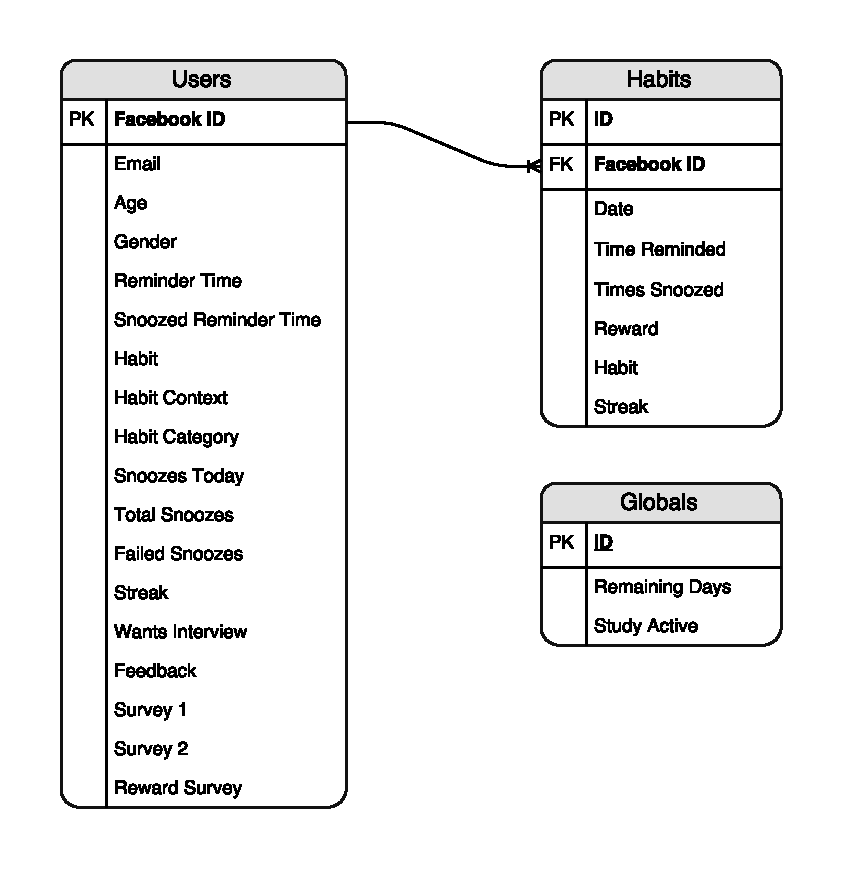
\includegraphics[width=5in]{../resources/diagrams/database-diagram.pdf}
    \caption{PostgreSQL Database entity table relationship diagram showing all information stored for Harry's Habits.}
    \label{fig:db_diagram}
\end{figure}


\subsection{Custom Application}
Figure~\ref{fig:prototype_detailed_overview} shows a detailed overview of the custom chatbot application and how it interacts with the database and the Facebook servers.

\begin{figure}[H]
    \centering
    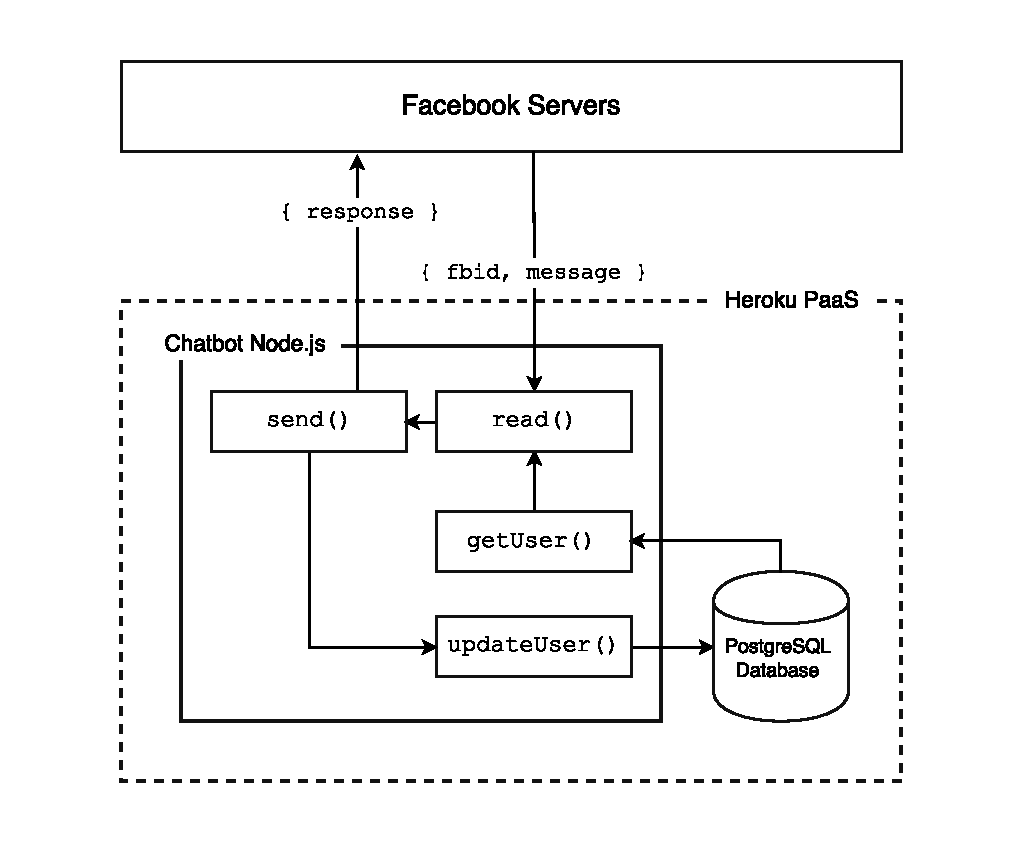
\includegraphics[width=6in]{../resources/diagrams/chatbot-detailed-overview.pdf}
    \caption{Overview of Harry's Habits interacting with Facebook servers to send and receive messages from the Messenger platform.}
    \label{fig:prototype_detailed_overview}
\end{figure}


When a user messages the chatbot on Facebook Messenger, the message is first sent to Facebook servers who make a HTTP request to a specified \textit{webhook URL} with a secret parameter for security. The chatbot handles this request then sends another with the same secret. The incoming HTTP request contains a payload with either a simple string of characters with a Facebook user ID (\textit{fbid}) or a Quick Reply key with a fbid. The chatbot application handles the incoming request with four components.

First, the \verb|read()| function checks if the incoming object is valid, then decides if it is a quick reply or just a regular message and strips the object of the unimportant parts until it is left with the fbid and either the message as a \verb|string| or the quick reply key.

Second, the \verb|getUser()| function uses the extracted fbid to collect information about the Facebook user from a PostgreSQL Database. If the fbid already exists in the database, it means the user has previously interacted with the chatbot, so details about that user are extracted from the \textit{Users} Table (Figure~\ref{fig:db_diagram}), e.g. the type of reward. Or if the user does not exist, it means the user has never interacted with the chatbot before.

Third, the \verb|send()| function decides what message to send back to the user. If this is the first time the user has messaged the chatbot, then a setup quick reply is created to start the setup flow (Section~\ref{setup_flow}). Otherwise based on the quick reply key or the individual message the chatbot will respond differently. For example, if a user sends `help' as a message, the application will prepare several messages to display a list of options users can choose and show more information about the bot. After the message is prepared, the application sends a request back to Facebook servers containing a regular message or a quick reply object with options and quick reply keys.

Finally after the message is sent, the \verb|updateUser()| will create a new row in the database if there is a new fbid, or it will update information about the user if they responded with a quick reply. For example, during the Trigger flow (Section~\ref{trigger_flow}) the chatbot asks users with a quick reply if they completed their habit. If a user marked a habit as completed, the message will have a quick reply key that the application can understand and a new row in the Habits Table will be created with that habit information.

\subsection{Delivering Rewards}

\begin{figure}[H]
    \centering
    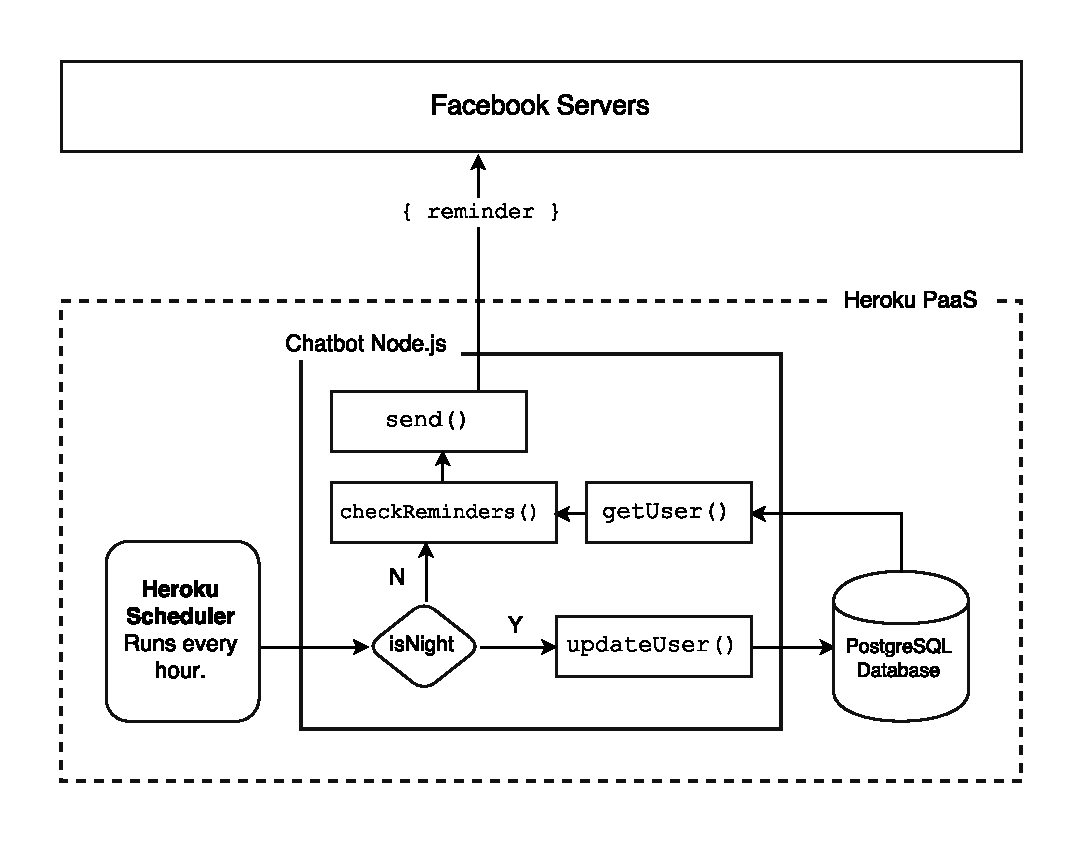
\includegraphics[width=6in]{../resources/diagrams/diagram-delivering-rewards.pdf}
    \caption{Overview of how notifications are sent by the application using a scheduler to check if it is time to send the notifications every hour.}
    \label{fig:prototype_sending_notifications}
\end{figure}

A notification is sent to a user just after the time of their habit context. Figure~\ref{fig:prototype_sending_notifications} shows how the Heroku scheduler (\url{https://elements.heroku.com/addons/scheduler}) handles this process by running a job on the chatbot application at scheduled intervals, similar to a cron job. It is scheduled to run every hour and run a node JavaScript file. This script first checks if the current time in UTC matches any of the 11 pre-defined times (Figure~\ref{fig:reminder_times}) and if it is, it reads the database to get information about all users that want to be sent a notification at that time. Then sends a quick reply message asking the user if they completed their habit or would like to be asked later (unless it is the night). If the later is chosen, the next reminder time later in the day is set to that user. Otherwise a reward is delivered.

\begin{figure}[H]
  \centering
\begin{lstlisting}
                       const reminderTimes = {
                           earlyMorning: 7,
                           midMorning: 9,
                           lateMorning: 11,
                           earlyAfternoon: 12,
                           midAfternoon: 14,
                           lateAfternoon: 16,
                           earlyEvening: 18,
                           midEvening: 20,
                           lateEvening: 21,
                           night: 22,
                           newDay: 23
                         };
\end{lstlisting}

  \caption{The JavaScript object that defines the scheduler times that users can set to receive post-completion notification.}
  \label{fig:reminder_times}
\end{figure}

The type of reward delivered is chosen when a user sends the `completed habit' quick reply response. The modality is based on the fbid of the user and is read from the database, then another message is delivered to that user containing the reward. A consistent method was built to deliver the reward to users, instead of sending the rewards in-line a \textit{webview} was used to display a website where users can open their reward. The website uses \textit{HTML}, \textit{CSS}, \textit{JavaScript} and also used server-side template rendering with \textit{Pug} (\url{www.pugjs.org}) and CSS preprocessing with \textit{SASS} (\url{www.sass-lang.com/}). The full source code is available on GitHub (\url{www.github.com/harrymt/harryshabits/tree/master/docs}). This also allowed us to break free of the Messenger chatbot sandbox and use \textit{HTML} elements to display the content in the same way, ensuring consistency across devices. The website could start the GIF or play the music or both for each reward type when a user pressed a button. Although this was not without limitations. The auditory reward would not stop playing when users closed the webview. This could be performed programatically, however during testing, would not always work. This was worked around by only playing the music for 15 seconds --- an appropriate time to view the reward. Auto-playing the auditory reward was not available when sending the audio in-line and the webview could use the \textit{HTML5} \verb|<audio>| element to enable auto-play.
But, for auto-play elements, the HTML5 standard needs a button press before it starts~\cite{mozilla_autoplay}.
This required another button to create a \textit{JavaScript} hook to auto-play.
However, during tests on low mobile data speeds, users found that they would have to press the button multiple times before the audio played.
This was because the audio would only play after it had loaded and created a lengthy delay, along with seemingly broken display.
Figure~\ref{fig:fast_slow_opening_rewards} describes the process of loading a reward on fast internet speeds and slow internet speeds. To create a better user experience, the button disappeared when pressed, using \textit{CSS} that would execute even if the audio hadn't loaded, and even on a poor connection.
Then JavaScript would execute after the page had fully loaded and play the audio if the button had already been pressed from the CSS, but if it hadn't then it would create a hook to play the audio after it had been pressed.
This ensured a seemly experience when using rewards for all levels of connection.

\begin{figure}[H]
    \centering
    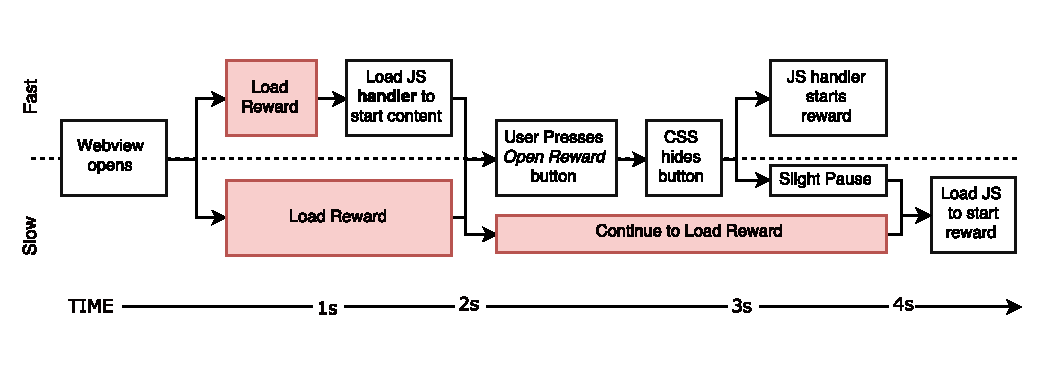
\includegraphics[width=6in]{../resources/diagrams/webview-flow-diagram.pdf}
    \caption{How rewards are displayed to the user when they are on fast internet (top lane) and slow internet (bottom lane) over time.}
    \label{fig:fast_slow_opening_rewards}
\end{figure}


\subsection{Testing and Continuous Integration}
To get a measure of code quality, several online services (codacy, codebeat and code climate) were used to track quality over time (see more on the GitHub repo \url{www.github.com/harrymt/harryshabits}). A test harness was also written to perform functional testing on the chatbot. An on-line continuous integration (CI) service (Travis CI) was used to programatically run these tests when a \textit{commit} in \textit{git} (the \textit{version control} used) was performed on the \textit{master branch}. \textit{Travis CI} (\url{https://travis-ci.org/harrymt/harryshabits}) ran the defined tests to ensure the functionality worked throughout development. A pilot trial with three users also tested the basic chatbot functionality preparing for the full evaluation study (Section~\ref{study_comparing_rewards}).

\subsection{Technical Issues}
Throughout the implementation process different techniques were explored to implement the design.
Some of the research areas were not used in the final prototype due to technical issues and limitations with the approach.

\subsubsection*{Habit Context Wording}
During the pilot trails users added the word `before' inside of their habit context (Figure~\ref{fig:study_bot_issues}). This resulted in messages being awkwardly worded, e.g. ``After 'before dinner' have you completed your daily press ups?''. This would be solved by adding another option to ask if they would like to perform it before or after, when asking for their habit context. Users also reported that after they snoozed the notifications several times, their habit context no longer became relevant, e.g. ``After 'eating lunch' have you completed your daily press ups?'' at 7pm. The context should be removed or altered in snoozed notifications. In addition, users should be asked if they want to change their context when being asked to change the time they receive their post-completion checks.

\begin{figure}[H]
  \centering
  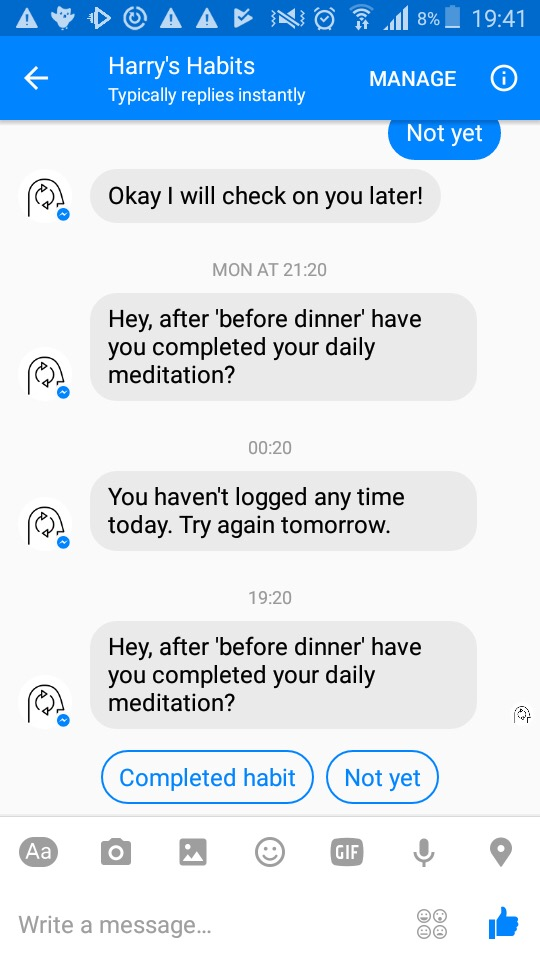
\includegraphics[width=2.1in]{../resources/feedback/after-before.jpg}
  \hspace{10px}
  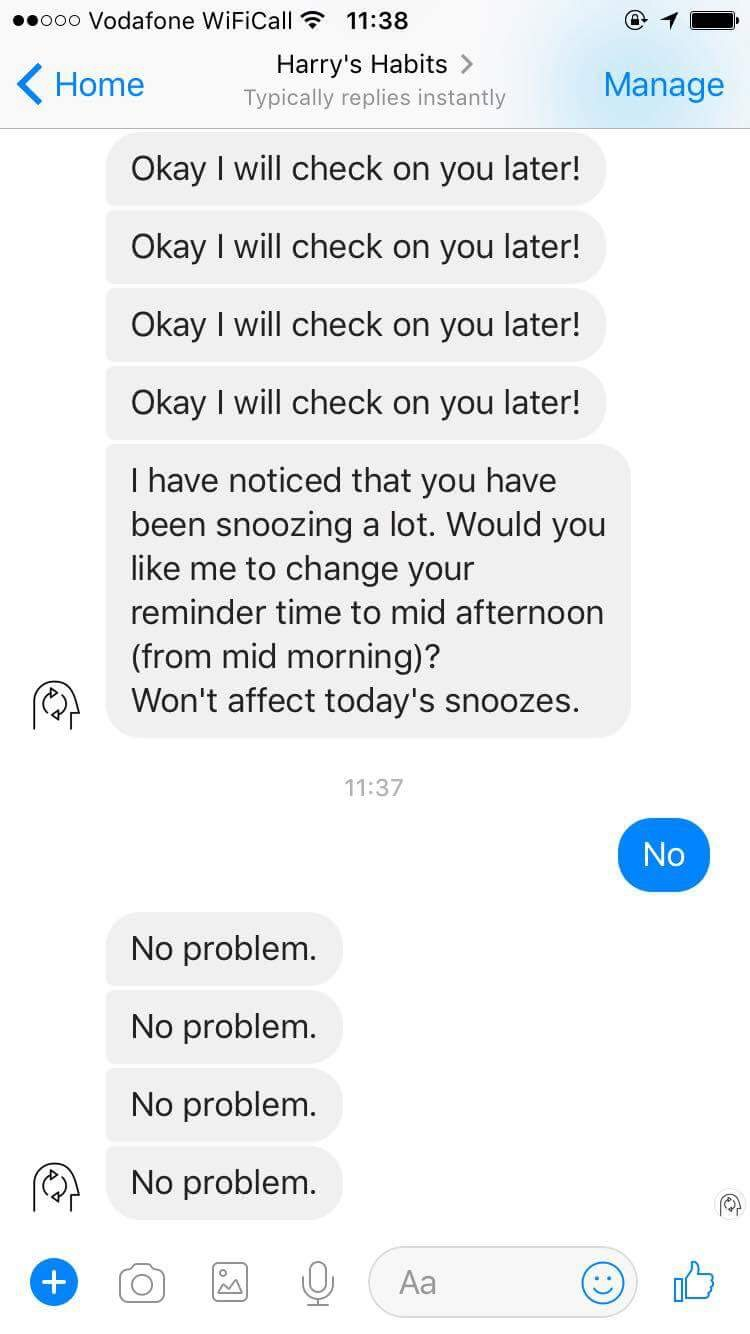
\includegraphics[width=2.1in]{../resources/feedback/double-messages.jpg}
  \caption{Example of 2 issues that occurred. First, the problem with habit context using the word `after'. Second, the bot sending the same message multiple times.}
  \label{fig:study_bot_issues}
\end{figure}

\subsubsection*{Message Interaction}
The chatbot would sometimes send multiple of the same message (Figure~\ref{fig:study_bot_issues}). This occurred when Facebook sent the same HTTP request multiple times. This could be helped by moving to a specific Facebook Messenger node JavaScript library module (\url{https://github.com/rickydunlop/fbmessenger-node}) to better suit interactions between Facebook servers and the app. This issue also effected another during the process of handling free text input from users. When the bot asked users to enter in a free text, e.g. email, a flag would be set to wait for free text input of that type. However, if duplicate messages were sent at this time, the application would assume users did not enter anything for the free text and would continue. Finally, if users accidentally sent the bot a message instead of responding to a quick reply, they would be unable to return to that quick reply menu and therefore breaking the flow of interaction. The question should be re-asked if it didn't fit the expected criteria.

\begin{figure}[H]
    \centering
    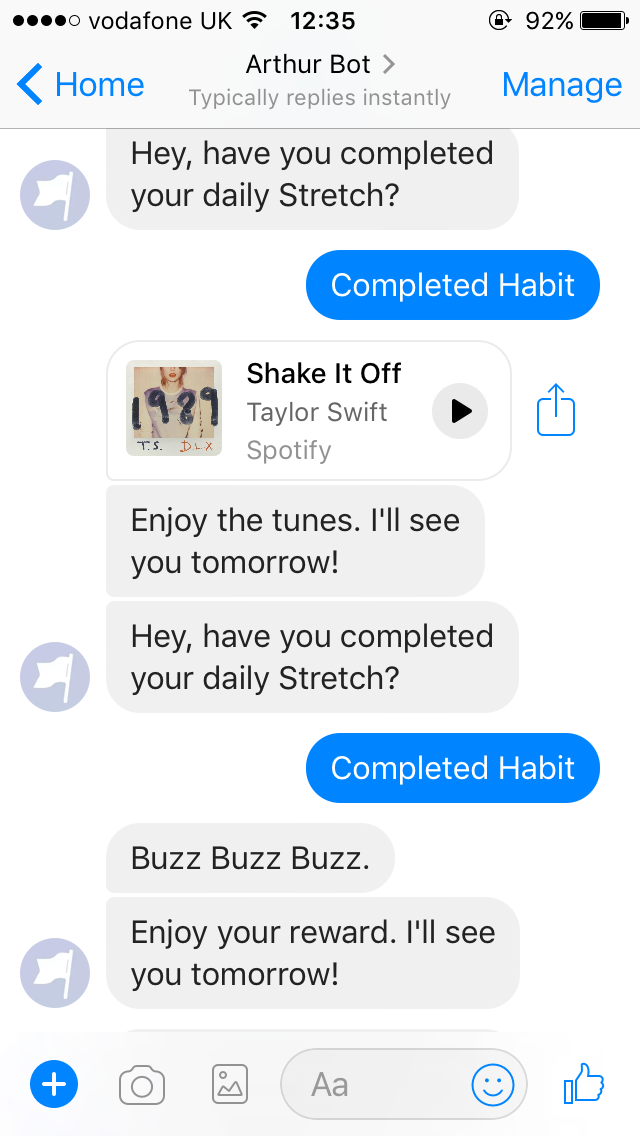
\includegraphics[width=1.8in]{../resources/design/vibration-reward.png}
    \caption{Using vibration as another modality was tested, but due to technical limitations was difficult to implement.}
    \label{fig:vibration_reward_issue}
\end{figure}

\subsubsection*{Vibration}
Using vibration as a modality would've been a great additional modality to use.
Unfortunately the chatbot sandbox meant that the vibration ability in the phone could not be used, so another device would be used in combination with the bot.
Smart watches and fitness trackers were researched to test if they could programatically vibrate, with the pattern of vibration matching the frequency of the audio.
However, the majority of these devices did not have an API that exposed the vibration element. The best method was found to programatically set an alarm 1-minute into the future using a Fitbit fitness tracker.
This would trigger the vibration when the alarm sounded.
Although this would mean a 1-minute delay after completing a habit, a good user flow could've reduced the wait time with some additional dialogue (Figure~\ref{fig:vibration_reward_issue}).
But, this approach relied on the fitness tracker to sync with the phone after the alarm was programatically set. Unfortunately forcing the tracker to sync wasn't available, so this modality was abandoned. Another issue occurred with stopping the audio after it had been played during a reward. If a user closed the reward box, there was no way to stop the audio, unless a user waited until it had finished. This limitation was very minor, but also showed how difficult it is to seemly connect a website and a chatbot. Finally, edge cases throughout interaction were revealed during development and were coded for, for example deciding what would happen if users snoozed their backup notification when it reached the end of the day led to additional logic to stop users from snoozing when it reached the end of the day.

\subsubsection*{Scheduler Time Zone}
The scheduler used had several limitations. First, the documentation stated it runs on a best effort basis and cannot guarantee to run on time, however, this did not affect the chatbot as it missed very few schedules. Second, the time zone of the scheduler had to be converted to Coordinated Universal Time (UTC) time before checking against the defined times. This issue was revealed in a pilot trail and fixed, however, for this application to work across different time-zones (ones that were not UTC), Figure~\ref{fig:reminder_times} would have to be custom to each user.

The implemented chatbot is tested during a 4-week study to answer the research questions and test the hypotheses.
\newpage
